% Original book diagram: fig:belief_space_geometry
% Book source: sections/Part_V/motion_planning.tex
% Original diagram authorship retained. Visual design: Ziad Mosalam.
\documentclass[11pt,border=8pt]{standalone}
\usepackage{amsmath,amssymb,graphicx,tikz}
\usetikzlibrary{arrows.meta,automata,positioning,calc,shapes.geometric,fit,backgrounds,patterns}
\newcommand{\vect}[1]{\mathbf{#1}}
\newcommand{\mat}[1]{\mathbf{#1}}
\newcommand{\Normal}{\mathcal{N}}
\newcommand{\prob}{p}
\newcommand{\E}{\mathbb{E}}
\newcommand{\Var}{\mathrm{Var}}
\newcommand{\Cov}{\mathrm{Cov}}
\newcommand{\CovP}{\mathbf{P}}
\newcommand{\Prob}{\mathbb{P}}
\setlength{\textwidth}{6.5in}
% Shared visual vocabulary for the book's original diagrams.
% Figures opt in explicitly, so unrelated text and existing additions are unchanged.
\definecolor{BookBlue}{HTML}{003262}
\definecolor{BookGold}{HTML}{B17A00}
\definecolor{BookTeal}{HTML}{247C86}
\definecolor{BookInk}{HTML}{30363B}
\definecolor{BookLight}{HTML}{E9EFF5}
\tikzset{
  book figure/.style={font=\small\rmfamily, color=BookBlue, text=BookInk,
    line width=0.8pt, >=Latex},
  book axis/.style={->, draw=BookInk, line width=0.6pt},
  book link/.style={->, draw=BookBlue, line width=0.8pt},
  book observation/.style={draw=BookGold, fill=BookGold!8},
  book state/.style={draw=BookBlue, fill=BookLight},
  book note/.style={font=\footnotesize\rmfamily, text=BookInk}
}

\begin{document}
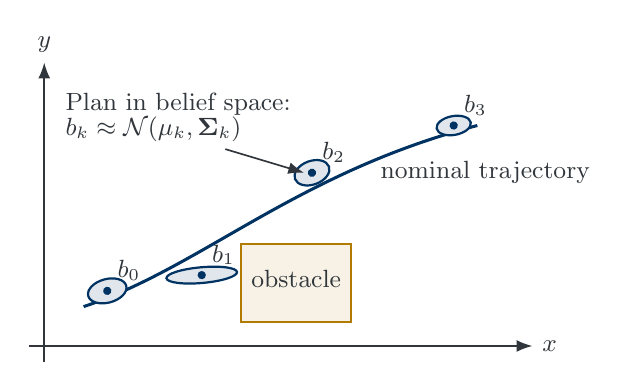
\begin{tikzpicture}[book figure, scale=1.0, >=Latex]
  % Axes
  \draw[book axis] (-0.2,0) -- (6.2,0) node[right] {$x$};
  \draw[book axis] (0,-0.2) -- (0,3.6) node[above] {$y$};

  % Nominal path
  \draw[BookBlue,line width=1.1pt] (0.5,0.5) .. controls (2.0,1.0) and (3.2,2.2) .. (5.5,2.8);
  \node at (5.6,2.2) {\small nominal trajectory};

  % Belief ellipses (covariance)
  \foreach \x/\y/\a/\b/\ang/\lab in {
    0.8/0.7/0.25/0.15/15/$b_0$,
    2.0/0.9/0.45/0.1/5/$b_1$,
    3.4/2.2/0.23/0.15/20/$b_2$,
    5.2/2.8/0.22/0.12/10/$b_3$
  }{
    \begin{scope}[shift={(\x,\y)}, rotate=\ang]
      \draw[BookBlue,fill=BookBlue!12] (0,0) ellipse [x radius={\a} , y radius={\b}];
      \fill (0,0) circle (1.5 pt);
    \end{scope}
    \node[above right] at (\x,\y) {\small \lab};
  }

  % Obstacles
  \fill[BookGold!10] (2.5,0.3) rectangle (3.9,1.3);
  \draw[BookGold] (2.5,0.3) rectangle (3.9,1.3);
  \node at (3.2,0.85) {\small obstacle};

  % Caption-like callouts
  \draw[book axis] (2.3,2.5) -- (3.3,2.2);
  \node[align=left] at (1.7,2.9) {\small Plan in belief space:\\[-2pt]
  \small $b_k \approx \Normal(\mu_k,\mat{\Sigma}_k)$};
\end{tikzpicture}
\end{document}
